\documentclass[a4paper]{article}

\usepackage{Sweave} %--------------------------------!
\usepackage{amsmath}
\usepackage{amssymb}
\usepackage{amsthm}
\usepackage{fancyhdr}
\usepackage[usenames, dvipsnames]{color}
\usepackage{verbatim}

\oddsidemargin 0cm
\topmargin -2.4cm     %I recommend adding these three lines to increase the
\textwidth 16.5cm   %amount of usable space on the page (and save trees)
\textheight 27.5cm

\newcommand{\question}[2] {\vspace{.25in} \hrule\vspace{0.5em}
\noindent{\bf #1: #2} \vspace{0.5em}
\hrule \vspace{.10in}}
\renewcommand{\part}[1] {\vspace{.10in} {\bf (#1)}}

\newcommand{\myname}{Xuan Han}
\newcommand{\myhusky}{han.xua@husky.neu}
\newcommand{\myhwnum}{6}

\setlength{\parindent}{0pt}
\setlength{\parskip}{5pt plus 1pt}

\pagestyle{fancyplain}
\lhead{\fancyplain{}{\textbf{HW\myhwnum}}}      % Note the different brackets!
\rhead{\fancyplain{}{\myname\\ \myhusky}}
\chead{\fancyplain{}{1 2}}


\begin{document}
\Sconcordance{concordance:category_response.tex:category_response.Rnw:%
1 45 1 1 2 1 0 2 1 3 0 1 2 1 1 1 2 1 0 10 1 1 2 1 1 1 2 5 0 1 4 33 1 1 %
2 1 0 11 1 1 2 5 1 10 0 1 1 19 0 1 5 35 1 1 2 1 0 1 1 26 0 1 2 7 1 1 2 %
1 0 3 1 4 0 1 2 5 1 1 2 8 0 1 2 6 1 1 2 1 0 1 1 7 0 3 1 6 0 1 1 6 0 1 2 %
6 1 1 2 8 0 1 2 2 1 1 2 1 0 3 1 9 0 1 2 4 1 1 2 1 0 4 1 8 0 1 2 6 1 1 2 %
4 0 1 2 1 1 1 2 1 0 3 1 1 2 4 1 4 0 1 2 4 1 1 2 1 0 3 1 4 0 1 2 6 1}


\title{Data Mining Assignment \myhwnum}
\author{\myname \\
        \myhusky}
\date{\today}
\maketitle

\thispagestyle{plain}


\question{1}{Employee}
\begin{Schunk}
\begin{Sinput}
> library(xtable)
> data = read.csv('performance.csv')
> attach(data)
\end{Sinput}
\end{Schunk}

\part{a}
\begin{Schunk}
\begin{Sinput}
> midX = median(X)
> group1 = subset(data, X >= midX)
> group2 = subset(data, X < midX)
> Y0count1 = sum(!group1$Y)
> Y1count1 = sum(group1$Y)
> Y0count2 = sum(!group2$Y)
> Y1count2 = sum(group2$Y)
> Q = c('aboveMid', 'belowMid')
> Y0Count = c(Y0count1, Y0count2)
> Y1Count = c(Y1count1, Y1count2)
> tableOfCount = data.frame(Q, Y0Count, Y1Count)
> Y0Prop = Y0Count / c(dim(group1)[1], dim(group2)[1])
> Y1Prop = Y1Count / c(dim(group1)[1], dim(group2)[1])
> tableOfProp = data.frame(Q, Y0Prop, Y1Prop)
> # xtable(tableOfCount, caption = 'tableOfCount')
> # xtable(tableOfProp, caption = 'tableOfProp')
\end{Sinput}
\end{Schunk}

\begin{table}[ht]
\centering
\begin{tabular}{rlrr}
  \hline
 & Q & Y0Count & Y1Count \\
  \hline
1 & aboveMid &   4 &  10 \\
  2 & belowMid &   9 &   4 \\
   \hline
\end{tabular}
\caption{tableOfCount}
\end{table}

\begin{table}[ht]
\centering
\begin{tabular}{rlrr}
  \hline
 & Q & Y0Prop & Y1Prop \\
  \hline
1 & aboveMid & 0.29 & 0.71 \\
  2 & belowMid & 0.69 & 0.31 \\
   \hline
\end{tabular}
\caption{tableOfProp}
\end{table}

{\color{red}
It's obvious from the table we can see that employees are tend to performe better when their emotion is more stable.\\
The propotion of emotion stability above median employees who can perform a task is almost twice as much as those who's emotion stablity is below median.
}


\part{b}
\begin{Schunk}
\begin{Sinput}
> quan = quantile(X)
> group1 = subset(data, X < quan[2] & X >= quan[1])
> group2 = subset(data, X < quan[3] & X >= quan[2])
> group3 = subset(data, X < quan[4] & X >= quan[3])
> group4 = subset(data, X >= quan[4])
> Q = c("Q1", "Q2", "Q3", "Q4")
> Y0Count = c(sum(!group1$Y), sum(!group2$Y), sum(!group3$Y), sum(!group4$Y))
> Y1Count = c(sum(group1$Y), sum(group2$Y), sum(group3$Y), sum(group4$Y))
> Y0prop = Y0Count / c(dim(group1)[1], dim(group2)[1], dim(group3)[1],dim(group4)[1])
> Y1prop = Y1Count / c(dim(group1)[1], dim(group2)[1], dim(group3)[1],dim(group4)[1])
> tableOfCount = data.frame(Q, Y0Count, Y1Count)
> tableOfProp = data.frame(Q, Y0prop, Y1prop)
> ys = c(6,1,3,3,3,4,1,6)
> cs = rep(c("Y0", "Y1"), 4)
> qs = rep(Q, 1, each = 2)
> temp = data.frame(ys, cs, qs)
> ov = xtabs(ys ~ qs + cs, data = temp)
> ov
\end{Sinput}
\begin{Soutput}
    cs
qs   Y0 Y1
  Q1  6  1
  Q2  3  3
  Q3  3  4
  Q4  1  6
\end{Soutput}
\begin{Sinput}
> prop.test(ov)
\end{Sinput}
\begin{Soutput}
	4-sample test for equality of proportions without continuity
	correction

data:  ov
X-squared = 7.2586, df = 3, p-value = 0.0641
alternative hypothesis: two.sided
sample estimates:
   prop 1    prop 2    prop 3    prop 4 
0.8571429 0.5000000 0.4285714 0.1428571 
\end{Soutput}
\begin{Sinput}
> # summary(ov)
> # xtable(tableOfCount, caption = 'tableOfCount')
> # xtable(tableOfProp, caption = 'tableOfProp')
\end{Sinput}
\end{Schunk}

\begin{table}[ht]
\centering
\begin{tabular}{rlrr}
  \hline
 & Q & Y0Count & Y1Count \\
  \hline
1 & Q1 &   6 &   1 \\
  2 & Q2 &   3 &   3 \\
  3 & Q3 &   3 &   4 \\
  4 & Q4 &   1 &   6 \\
   \hline
\end{tabular}
\caption{tableOfCount}
\end{table}

% \begin{table}[ht]
% \centering
% \begin{tabular}{rlrr}
%   \hline
%  & Q & Y0prop & Y1prop \\
%   \hline
% 1 & Q1 & 0.86 & 0.14 \\
%   2 & Q2 & 0.50 & 0.50 \\
%   3 & Q3 & 0.43 & 0.57 \\
%   4 & Q4 & 0.14 & 0.86 \\
%    \hline
% \end{tabular}
% \caption{tableOfProp}
% \end{table}
{\color{red}
p-value of Pearson X-squared test is 0.064, null hypothesis rejected, which means there is association between X and Y, which is in consistant with (a).
}


\part{c}
\begin{Schunk}
\begin{Sinput}
> fit = glm(Y ~ X, family = binomial, data)
> summary(fit)
\end{Sinput}
\begin{Soutput}
Call:
glm(formula = Y ~ X, family = binomial, data = data)

Deviance Residuals: 
    Min       1Q   Median       3Q      Max  
-1.7845  -0.8350   0.5065   0.8371   1.7145  

Coefficients:
              Estimate Std. Error z value Pr(>|z|)  
(Intercept) -10.308925   4.376997  -2.355   0.0185 *
X             0.018920   0.007877   2.402   0.0163 *
---
Signif. codes:  0 ‘***’ 0.001 ‘**’ 0.01 ‘*’ 0.05 ‘.’ 0.1 ‘ ’ 1

(Dispersion parameter for binomial family taken to be 1)

    Null deviance: 37.393  on 26  degrees of freedom
Residual deviance: 29.242  on 25  degrees of freedom
AIC: 33.242

Number of Fisher Scoring iterations: 4
\end{Soutput}
\end{Schunk}
{\color{red}
Assumtion:\\
Y are Benoulli random variables, independent, and P\{Y=1\} is related to X according to the specified logistic function.\\
As we can see from the summary, $\beta_1$ is 0.0189. The intercept is -10.3.
}


\part{d}
\begin{Schunk}
\begin{Sinput}
> new.x = data.frame(X = seq(300, 1000))
> new.y <- predict(fit, newdata = new.x, se.fit=T, type="response")
> plot(X, Y, col = rainbow(7))
> lines(new.x$X, new.y$fit, col = "blue")
\end{Sinput}
\end{Schunk}
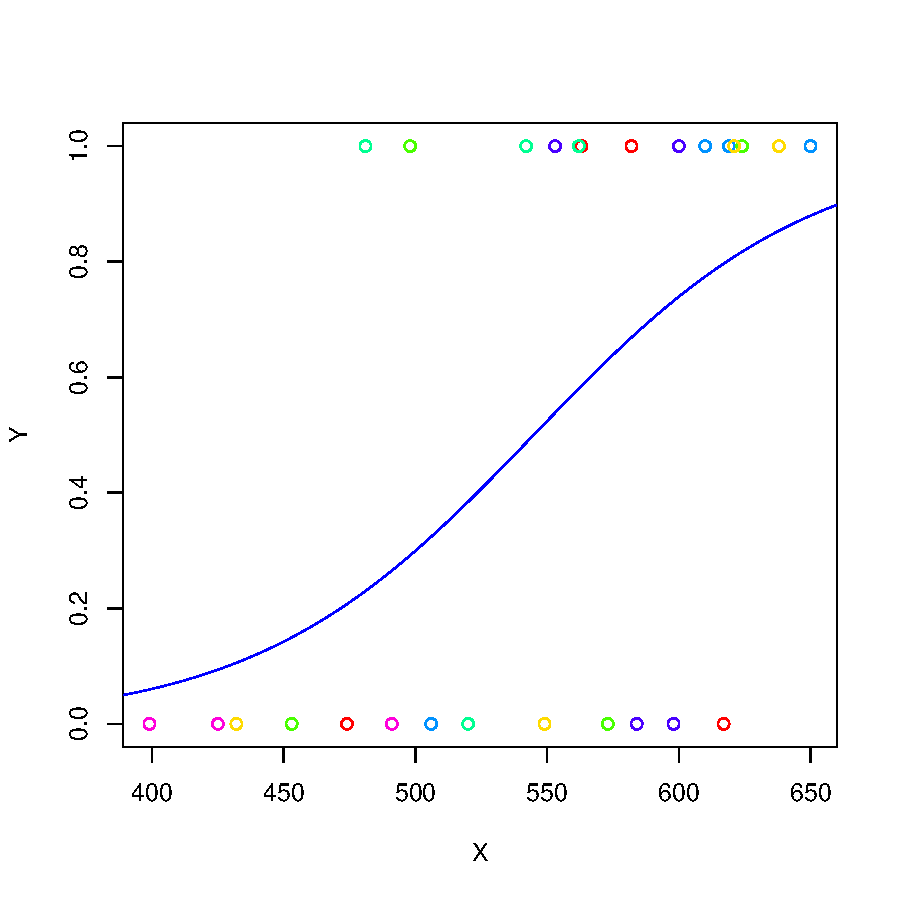
\includegraphics{category_response-1d}
{\color{red}\\
From the plot, I might say that the model fit is OK.\\
But we can also see that there are lots of overlap from 450 to 600, so the model might not work well in this range.
}

\part{e}
\begin{Schunk}
\begin{Sinput}
> fit$coefficients
\end{Sinput}
\begin{Soutput}
 (Intercept)            X 
-10.30892518   0.01891983 
\end{Soutput}
\end{Schunk}
{\color{red}
Since we get $\beta_1 = 0.0189$ and its SE is only 0.0078 and its p-value is 0.0163, we are sure that there is association between X and Y.\\
And the increase of log-odds of P\{Y=1\} with unit increase of X is 0.0189.\\
This means that there is a positive association between X and Y. The bigger X, the more likely that Y is 1. This is in constant with (a) and (b)
}

\part{f}
\begin{Schunk}
\begin{Sinput}
> interval = confint(fit, level = c(0.9))
> interval
\end{Sinput}
\begin{Soutput}
                      5 %        95 %
(Intercept) -18.628406505 -3.90734449
X             0.007348506  0.03382477
\end{Soutput}
\begin{Sinput}
> intervalX = c(interval[2, 1], interval[2, 2])
> e.beta1 = exp(intervalX)
> exp(fit$coefficients[2])
\end{Sinput}
\begin{Soutput}
     X 
1.0191 
\end{Soutput}
\begin{Sinput}
> e.beta1
\end{Sinput}
\begin{Soutput}
[1] 1.007376 1.034403
\end{Soutput}
\end{Schunk}
{\color{red}
We get $e^{\beta_1} = 1.0191$ and its 95\% confident interval.\\
This interval of e.beta1 means that: \\
with 95\% probability, unit increase in X will lead to odds of P\{Y=1\} increase by at minimum 1.007376 and at maximum 1.034403.
}

\part{g}
\begin{Schunk}
\begin{Sinput}
> predict(fit, data.frame(X = c(550)), type = "res")
\end{Sinput}
\begin{Soutput}
        1 
0.5242263 
\end{Soutput}
\end{Schunk}


\part{h}
\begin{Schunk}
\begin{Sinput}
> pred.prob = predict(fit, data, type = "res")
> pred.label = rep(0, 27)
> pred.label[pred.prob > 0.5] = 1
> table(pred.label, Y)
\end{Sinput}
\begin{Soutput}
          Y
pred.label  0  1
         0  8  3
         1  5 11
\end{Soutput}
\end{Schunk}
{\color{red}
We can see that there are 11 true positives, 8 true negatives, 5 false positives and 3 false negatives.
}

\part{i}
\begin{Schunk}
\begin{Sinput}
> library(ROCR)
> pred <- prediction(pred.prob, labels = Y)
> perf <- performance(pred, "tpr", "fpr")
> plot(perf, colorize=F, main = "ROC curve")
> attributes(performance(pred, "auc"))$y.values
\end{Sinput}
\begin{Soutput}
[[1]]
[1] 0.7967033
\end{Soutput}
\end{Schunk}
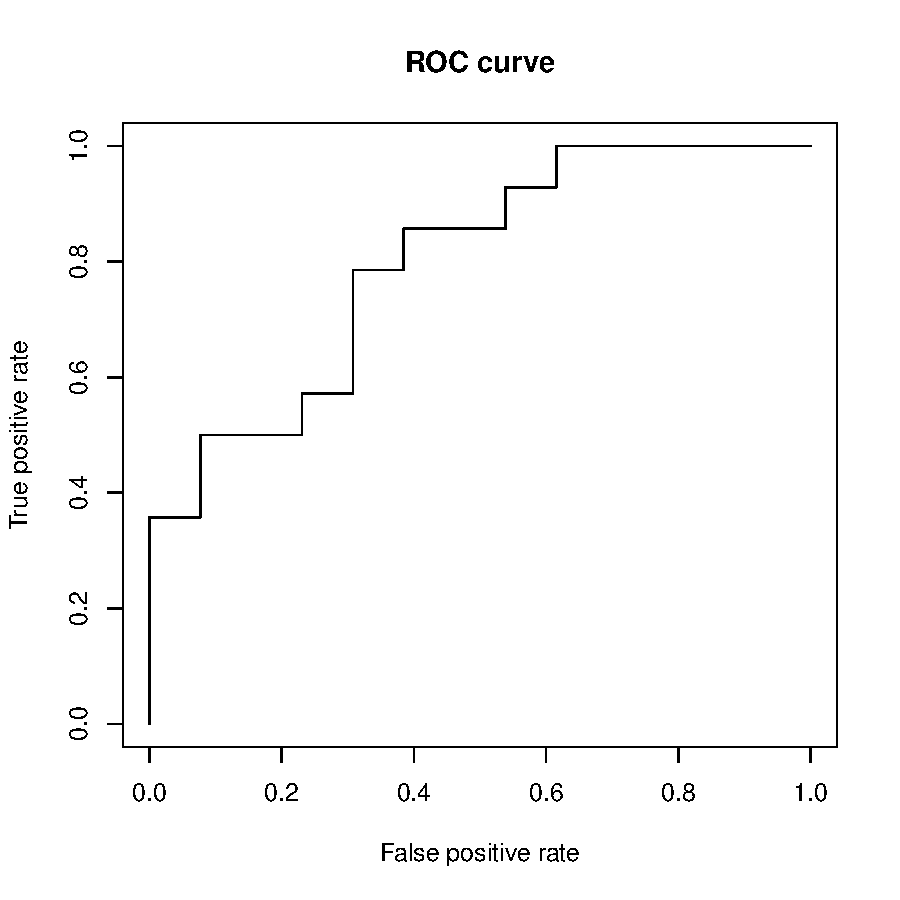
\includegraphics{category_response-1i}
{\color{red}\\
First, we can see that TPR increase with FPR. And they both reach 1.0 at upper-right corner.\\
We can see that the AUC is 0.7967, which means that the model is on the right track, but not a very good job.
}


\question{2}{Experiment}
\begin{Schunk}
\begin{Sinput}
> x = seq(from = -10, to = 200, length = 500)
\end{Sinput}
\end{Schunk}

\part{a}
\begin{Schunk}
\begin{Sinput}
> beta0 = -25
> beta1 = 0.2
> y1 = 1 / (1 + exp(-beta0 - beta1 * x))
> plot(y1 ~ x, col = 'red', type = 'l')
> beta11 = 2
> y2 = 1 / (1 + exp(-beta0 - beta11 * x))
> lines(y2 ~ x, col = 'green')
> title('sigmoid')
> legend('bottomright', legend = c('beta1=0.2', 'beta1=2'), col = c('red', 'green'), pch = 1:1)
\end{Sinput}
\end{Schunk}
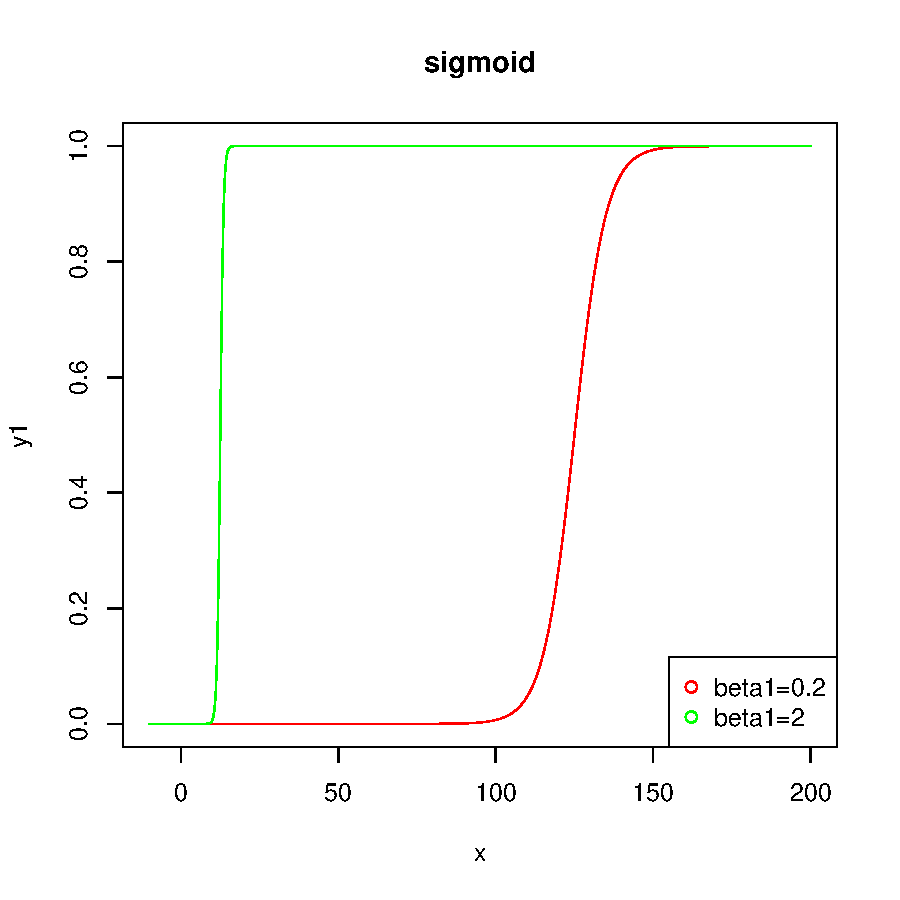
\includegraphics{category_response-2a}
{\color{red}\\
From the plot we can see that with a bigger $\beta_1$, the curve tends to be more steep and y reach 1 eailer. This is because $\beta_1$ represents the change speed of log-odds of y = 1. With a bigger $\beta_1$, the log-odds becomes bigger. So y tends to reach 1 more quickly.
}

\part{b}
\begin{Schunk}
\begin{Sinput}
> beta2 = -2
> y3 = 1 / (1 + exp(-beta0 - beta1 * x - beta2 * I(x ^ 2)))
> plot(y3 ~ x, col = 'red', type = 'l')
> title('sigmoid')
\end{Sinput}
\end{Schunk}
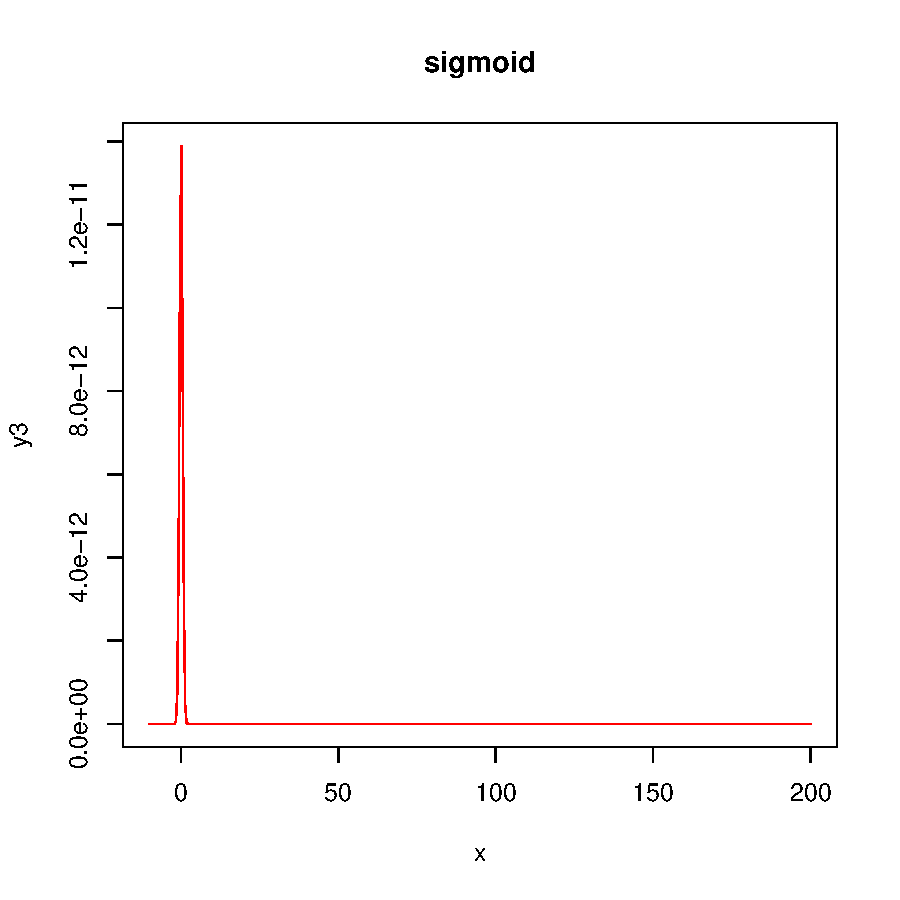
\includegraphics{category_response-2b}

{\color{red}
This plot is somewhat looks abnormal.\\ But what it tells us is that $X^2$ and Y has a strong negative association, and this association dominate. When x goes from -10 to 0, $X^2$ becomes smaller so y goes up; When x passes 0, $X^2$ becomes bigger, y goes down, until 0.
}


\end{document}
